\documentclass[11pt,letter]{article}
\usepackage[top=1.00in, bottom=1.0in, left=1.1in, right=1.1in]{geometry}
\usepackage{Sweave}
\renewcommand{\baselinestretch}{1.1}
\usepackage{graphicx}
\usepackage{natbib}
\usepackage{amsmath}
\usepackage{xr}
\externaldocument{phencc}

\def\labelitemi{--}
\parindent=0pt

\begin{document}

\renewcommand{\refname}{\CHead{}}

\title{Supplemental materials:  How environmental tracking shapes communities in stationary \& non-stationary systems} 

\author{E. M. Wolkovich \& M. J. Donohue}
\date{} 
\maketitle  %put the fancy title on
\renewcommand{\thetable}{S\arabic{table}}
\renewcommand{\thefigure}{S\arabic{figure}}

\section{Literature review}
We systematically reviewed the literature for studies examining tracking and other traits. We searched ISI in August 2019 for:
\begin{enumerate}
\item Topic: `phenolog* chang*' and Title: phenolog* AND trait*
\item Topic: `warming shift*' AND trait* and Title: phenolog*
\item Topic: `phenolog* track*' AND trait* and Title: phenolog*
\item Topic: `phenolog* sensitiv*' AND trait* and Title: phenolog*
\end{enumerate}
which resulted in 231 papers. From here we used the following criteria to determine from which papers we could not extract data: no phenology or phenological change measured (73 papers), no trait(s) measured or analyzed (49 papers), single-species studies focused on intra-specific variation (54 papers), modeling or theory studies without data (12 papers), or papers without new data presented (reviews, etc.: 4 papers), or miscellaneous reasons leading to no data relevant to our aims (7 papers). This left us with 30 papers including relevant data \citep{Suzuki:1997gf,Post1999,adrian2006,Xu:2009an,Goodenough2010,Diamond:2011nx,Moussus2011,Szilvia2012,Dorji2013,Ishioka2013,xia2013,Bock2014,kharouba2014,Vegvari2015,bell2015,lasky2016,McDermott2016,Zhu2016BioLetters,brooks2017,du2017,munson2017,arfinkhan2018,zhang2018,Ladwig2019,park2019,,sharma2019,Xavier2019,Zettlemoyer2019}, eight of which did not test for a relationship between tracking and the other studied traits \citep{Suzuki:1997gf,adrian2006,Xu:2009an,bell2015,McDermott2016,Sherwood2017,sharma2019,Xavier2019}. We present data from the remaining papers in Tables \ref{tab:meta1}-\ref{tab:meta2}. Most studies examined tracking as how a phenophase related to temperature (86\% of all tracking metrics), followed by precipitation (10\%, includes snow removal), followed by photoperiod (3\%), followed by the climate mode NAO (1\%) and water table depth (0.5\%). Four of the 30 studies examined more than one major climate metric, though some measured many versions of temperature and/or precipitation metrics \citep[e.g., 15 precipitation and/or temperature metrics considered in][]{munson2017}.

% Could add why my review was not included (no tracking) and not including Brown review ... 
% Should add average number of traits and phenophases in each study. It was a mode of one for both phenophases and traits ... 

\newpage 
\clearpage
\section{Model}

\begin{center}
\begin{table}[h!]
\caption{Table of parameter values, their definitions and lightweight version of their dimensions (i.e., not yet deemed `grams' or such).}
\begin{tabular}{ | p{3.0cm} | p{6.0cm} | p{4.0cm} |}
\hline 
Parameter & Definition & Unit \\ \hline 
\end{tabular}
\begin{tabular}{ | p{3.0cm} | p{6.0cm} | p{4.0cm} |}
\(N_{i}\) & seedbank of species \(i\) & seeds \\ \hline
\(s_{i}\) & survival of species \(i\) & unitless \\ \hline
\(\delta\) (peak biomass) & total length of growing season & days\\ \hline
\(B_{i}\) & biomass of species \(i\) & biomass \\ \hline
\(R\) & resource & resource\\ \hline
\(c_{i}\) & conversion of \(R\) uptake to biomass of species \(i\) &  \(\frac{\text{biomass}}{\text{resource}}\) \\ \hline
\(m_{i}\) & maintenance costs of species \(i\) & \(\text{days}^{-1}\) \\ \hline
\(a_{i}\) & uptake increase as \(R\) increases for species \(i\) & \(\text{days}^{-1}\) \\ \hline
\(u_{i}\) & max uptake for species \(i\) & \(\frac{(\text{days})(\text{biomass})}{\text{resource}}\) \\ \hline
\(\phi_{i}\) & converesion of biomass to seedbank for species, includes overwintering of seeds \(i\) & \(\text{biomass}^{-1}\), but conceptually \(\frac{\text{seeds}}{(\text{biomass})(\text{seeds})}\) \\ \hline
\(\epsilon\) & abiotic loss of \(R\) &  \(\text{days}^{-1}\) \\ \hline
\(g_{max,i}\) & max germination of species \(i\) & unitless \\ \hline
\(h_{i}\) &  controls the the rate at which germination declines as \(\tau_{p}\) deviates from optimum for species \(i\)  & \(\text{days}^{-2}\) \\ \hline
\(g_{i}\) & germination fraction & unitless \\ \hline
\(\tau_{p}\) & timing of pulse & days \\ \hline
\(\tau_{i}\) & timing of max germination of species \(i\) & days \\ \hline
\(\alpha_{i}\) & phenological tracking of species \(i\) & unitless \\ \hline
\(\theta_{i}\) & shape of uptake for species \(i\) & unitless\\ \hline
\hline
\(b_{i}\) & seedling biomass of species \(i\) & \(\frac{\text{biomass}}{\text{seeds}}\) \\ \hline
\(f_{i}(R)\) & \(R\) uptake \(f(x)\) for species \(i\) & \(\frac{\text{resource}}{(\text{days})(\text{biomass})}\)\\ \hline
\(d_{i}\) & death rate of species \(i\), used in calculations of lifespan & unitless \\ \hline
\(t\) & between year time (formerly T) & years \\ \hline
\(0\) $\rightarrow$ \(\delta\) & within season time (formerly \(\tau\)) & days \\ \hline
\(b_{0}\) & initial biomass per germinant (seed) & biomass \\ \hline
\(\xi\) & \(\frac{\text{final biomass}}{\text{initial biomass}}\) & unitless \\ \hline
\hline
\end{tabular}
\end{table}
\end{center}

\bibliography{/Users/Lizzie/Documents/git/bibtex/LizzieMainMinimal}
\bibliographystyle{/Users/Lizzie/Documents/git/bibtex/styles/ecolett.bst}


\clearpage
\begin{figure}[t!]
\centering
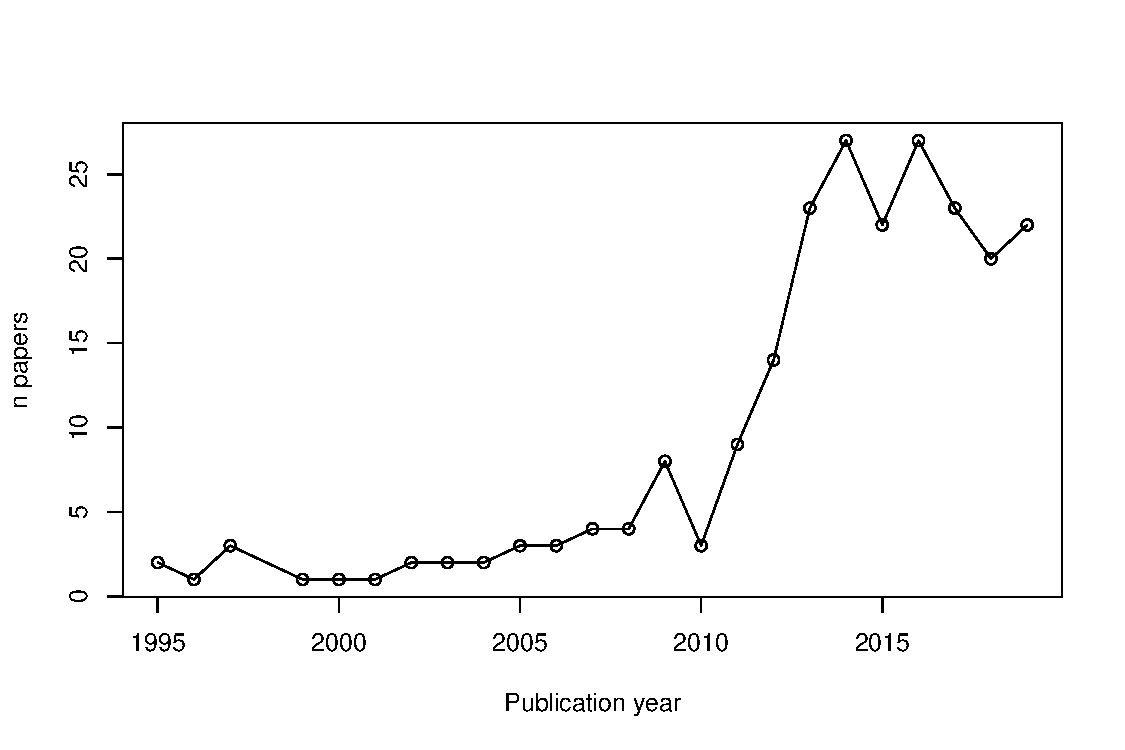
\includegraphics[width=1\textwidth]{..//..//R/graphs/otherdat/papersovertime.pdf}
\caption{Trends in all papers using search terms over time. Of papers from which we could extract data all were published in 2016 or onward.}
  \label{fig:papertrends}
\end{figure}
 
 \newpage
% latex table generated in R 3.5.1 by xtable 1.8-3 package
% Sat Oct 12 17:16:43 2019
\begin{table}[ht]
\centering
\caption{Summary of traits related to phenological tracking in the literature and whether papers reported statistical evidence that they were linked or not. See Table S2 for an extended version.} 
\label{tab:meta1}
\begingroup\footnotesize
\begin{tabular}{lrr}
  \hline
Trait & n linked & n not linked \\ 
  \hline
diet traits &   0 &   4 \\ 
  early/late phenophase &  10 &   4 \\ 
  habitat traits &   1 &   4 \\ 
  height &   1 &   0 \\ 
  hibernation stage &   0 &   4 \\ 
  leaf/shoot size &   1 &   0 \\ 
  migration traits &   3 &   3 \\ 
  mobility &   1 &   3 \\ 
  nativeness &   1 &   3 \\ 
  niche breadth &   3 &   2 \\ 
  other Lepidopteran traits &   3 &   4 \\ 
  other bird traits &   1 &   1 \\ 
  other leaf traits &   4 &   3 \\ 
  other plant traits &   1 &   1 \\ 
  overwintering &   2 &   1 \\ 
  range traits &   1 &   4 \\ 
  root traits &   3 &   0 \\ 
  seed weight/size/number &   1 &   2 \\ 
  woody/herbaceous &   1 &   0 \\ 
   \hline
\end{tabular}
\endgroup
\end{table}% latex table generated in R 3.5.1 by xtable 1.8-3 package
% Sat Oct 12 17:16:43 2019
\begin{table}[ht]
\centering
\caption{Summary of results from literature on phenological tracking showing which phenophases researchers found were linked to which traits, or not.} 
\label{tab:meta2}
\begingroup\footnotesize
\begin{tabular}{lllrr}
  \hline
Taxa & Phenophase & Trait & n linked & n not linked \\ 
  \hline
Lepidoptera & activity length & hibernation stage &  &   1 \\ 
  Lepidoptera & activity length & migration traits &  &   1 \\ 
  Lepidoptera & activity length & other Lepidopteran traits &   1 &  \\ 
  Lepidoptera & appearance/collection date & diet traits &  &   1 \\ 
  Lepidoptera & appearance/collection date & early/late phenophase &   2 &  \\ 
  Lepidoptera & appearance/collection date & habitat traits &  &   2 \\ 
  Lepidoptera & appearance/collection date & hibernation stage &  &   1 \\ 
  Lepidoptera & appearance/collection date & migration traits &   1 &  \\ 
  Lepidoptera & appearance/collection date & mobility &  &   2 \\ 
  Lepidoptera & appearance/collection date & niche breadth &   2 &   1 \\ 
  Lepidoptera & appearance/collection date & other Lepidopteran traits &   1 &   2 \\ 
  Lepidoptera & appearance/collection date & overwintering &   2 &  \\ 
  Lepidoptera & appearance/collection date & range traits &   1 &   2 \\ 
  Lepidoptera & flight timing & early/late phenophase &   1 &   1 \\ 
  Lepidoptera & flight timing & mobility &   1 &   1 \\ 
  Lepidoptera & flight timing & niche breadth &  &   1 \\ 
  Lepidoptera & flight timing & other Lepidopteran traits &  &   1 \\ 
  Lepidoptera & flight timing & overwintering &  &   1 \\ 
  Lepidoptera & flight timing & range traits &  &   1 \\ 
  Lepidoptera & last/median emergence dates & diet traits &  &   2 \\ 
  Lepidoptera & last/median emergence dates & habitat traits &  &   2 \\ 
  Lepidoptera & last/median emergence dates & hibernation stage &  &   2 \\ 
  Lepidoptera & last/median emergence dates & migration traits &  &   2 \\ 
  Lepidoptera & last/median emergence dates & other Lepidopteran traits &   1 &   1 \\ 
  passerine birds & breeding time & diet traits &  &   1 \\ 
  passerine birds & breeding time & habitat traits &   1 &  \\ 
  passerine birds & breeding time & migration traits &   2 &  \\ 
  passerine birds & breeding time & niche breadth &   1 &  \\ 
  passerine birds & breeding time & other bird traits &   1 &   1 \\ 
  plants & budbreak/leafing & early/late phenophase &   3 &   1 \\ 
  plants & budbreak/leafing & nativeness &  &   1 \\ 
  plants & budbreak/leafing & other leaf traits &   2 &   1 \\ 
  plants & budbreak/leafing & range traits &  &   1 \\ 
  plants & flowering/fruiting & early/late phenophase &   4 &   2 \\ 
  plants & flowering/fruiting & height &   1 &  \\ 
  plants & flowering/fruiting & leaf/shoot size &   1 &  \\ 
  plants & flowering/fruiting & nativeness &   1 &   2 \\ 
  plants & flowering/fruiting & other leaf traits &   2 &   2 \\ 
  plants & flowering/fruiting & other plant traits &   1 &   1 \\ 
  plants & flowering/fruiting & root traits &   3 &  \\ 
  plants & flowering/fruiting & seed weight/size/number &   1 &   2 \\ 
  plants & flowering/fruiting & woody/herbaceous &   1 &  \\ 
   \hline
\end{tabular}
\endgroup
\end{table}

\clearpage
\begin{figure}[t!]
\centering
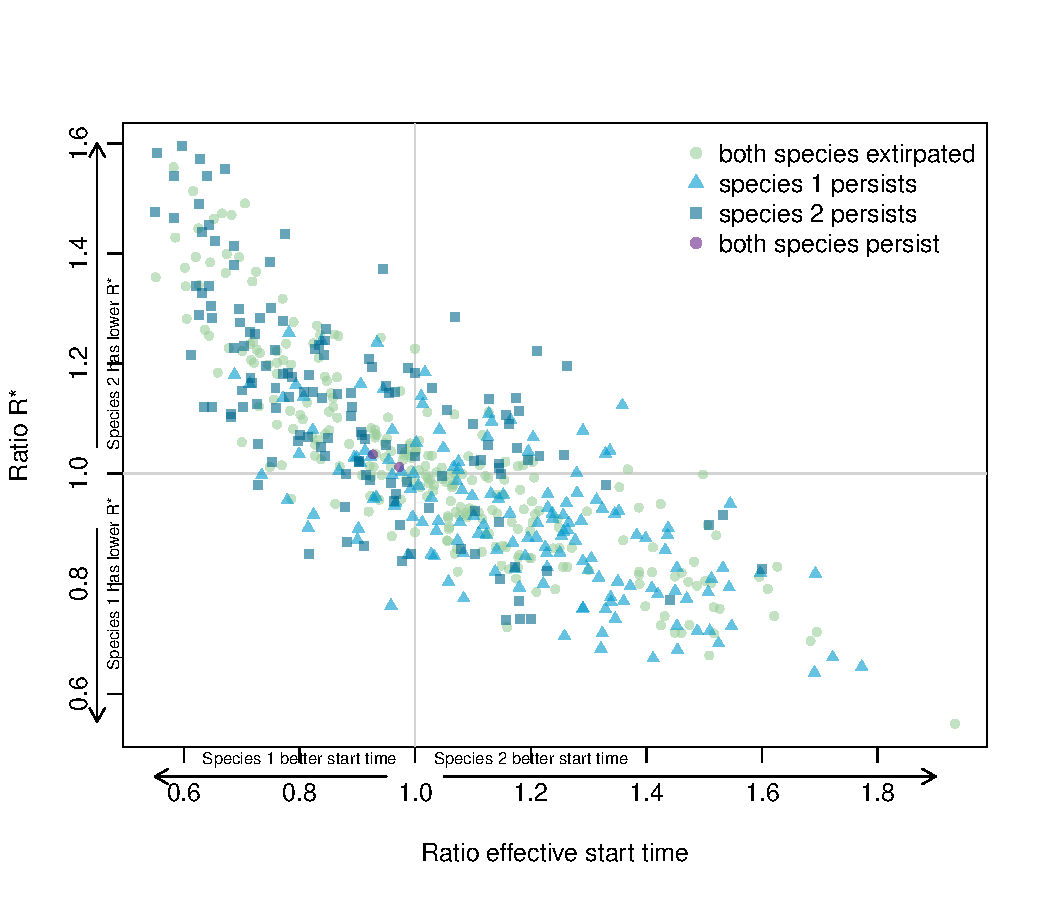
\includegraphics[width=0.9\textwidth]{..//..//R/graphs/modelruns/manuscript/tauIPrstart1.pdf}
\caption{How non-stationarity reshapes two-species communities in a simple model where effective start time (X axis: species 1/species 2) trades off with $R^*$ (Y axis: species 1/species 2): each point represents one two-species community that persisted through 500 years of stationary dynamics while the shape and color represent the outcome for that two-species community of 500 years of non-stationarity, where the abiotic start of the season shifts earlier.}
 \label{fig:tauirstarsupp}
\end{figure}


\begin{figure}[t!]
\centering
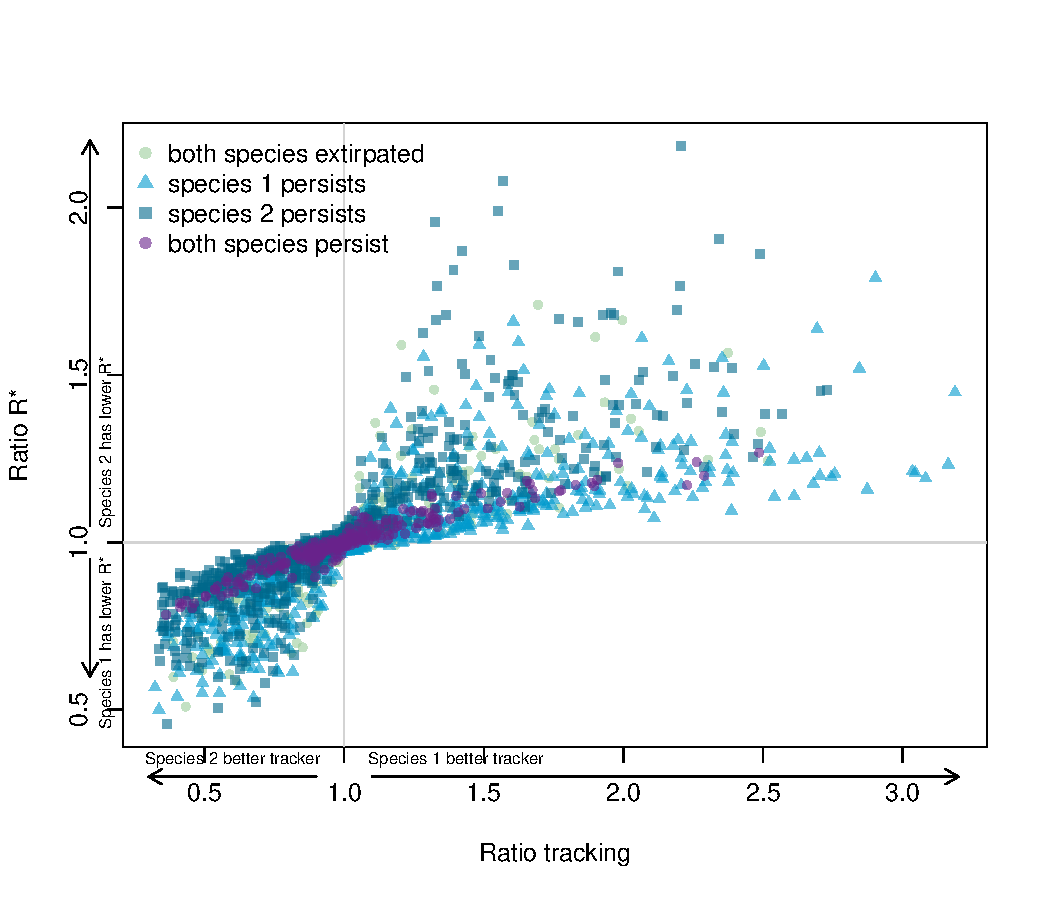
\includegraphics[width=0.9\textwidth]{..//..//R/graphs/modelruns/manuscript/alpharstar.pdf}
\caption{How non-stationarity reshapes two-species communities in a simple model where tracking (X axis: species 1/species 2) trades off with $R^*$ (Y axis: species 1/species 2): each point represents one two-species community that persisted through 500 years of stationary dynamics while the shape and color represent the outcome for that two-species community of 500 years of non-stationarity, where the abiotic start of the season shifts earlier.}
\label{fig:alpharstarsupp}
\end{figure}

\end{document}

\section{Model runs}

\emph{Analyses}: Ran XX models ...
